\documentclass[
titlepage=firstiscover,
bibliography=totoc,
captions=tableheading,
]{scrartcl}

\usepackage[aux]{rerunfilecheck}



\usepackage{polyglossia}
\usepackage[autostyle]{csquotes}
\setmainlanguage{german}
\setotherlanguages{english, french}

\usepackage{microtype}

\usepackage{amsmath}
\usepackage{amssymb}
\usepackage{mathtools}

\usepackage{fontspec}

\usepackage[
  style=alphabetic,
]{biblatex}
\addbibresource{main.bib}

\usepackage[
math-style=ISO,
bold-style=ISO,
sans-style=italic,
nabla=upright,
partial=upright,
]{unicode-math}

\usepackage[
  locale=DE,
  separate-uncertainty=true,
  per-mode=symbol-or-fraction,
]{siunitx}

\sisetup{
locale=DE,
per-mode=symbol-or-fraction}

\usepackage[unicode]{hyperref}
\usepackage{bookmark}

\usepackage{graphicx}
\graphicspath{{build/}}

\usepackage{caption, booktabs}

\usepackage{grffile}
\usepackage{subcaption}
\usepackage{float}

\usepackage{xfrac}


\begin{document}

  \section{Aufgabe 1}

    \subsection{Aufgabe 1a}

      Es werden zunächst $10⁵$ Zufallszahlenpaare in einem Kasten erzeugt,
      welcher in $x$-Richtung die Grenzen 0 und 20 hat und in
      $y$-Richtung von 0 und $y_{max}$ begrenzt wird.\\
      $y_{max}$ ist der maximale $y$-Wert der Verteilung
      lässt sich berechnen, indem von
      \begin{align*}
        f'(x)=\frac{Nx²}{e^x-1}\left(3-\frac{xe^x}{e^x-1}\right)
      \end{align*}
      (also der Ableitung der Planck-Verteilung) die Nullstelle
      mit scipy.optimize.brentq berechnet wird. Der zur Nullstelle
      gehörige $y$-Wert ist dann $y_{max}$ und liegt hier bei etwa 0.22.\\
      Aus diesen Zufallszahlenpaaren werden diejenigen ausgewählt, die unter
      der Planck-Kurve liegen. Der Rest wird zurückgegeben. Es werden so
      viele neue Zufallszahlenpaare erzeugt, wie alte zurückgegeben wurden.
      Mit diesen wird das Verfahren wiederholt. Insgesamt wird das
      Verfahren so lange fortgeführt, bis alle $10⁵$ Zufallszahlenpaare
      unter der Planck-Kurve liegen. \\
      Plottet man diese Paare, entsteht ein Bild wie in Abb. \ref{fig:planck},
      in welchem die Fläche unter der Planck-Kurve nahezu vollständig
      von Punkten ausgefüllt ist und die restliche Fläche frei ist.

      \begin{figure}[H]
        \centering
        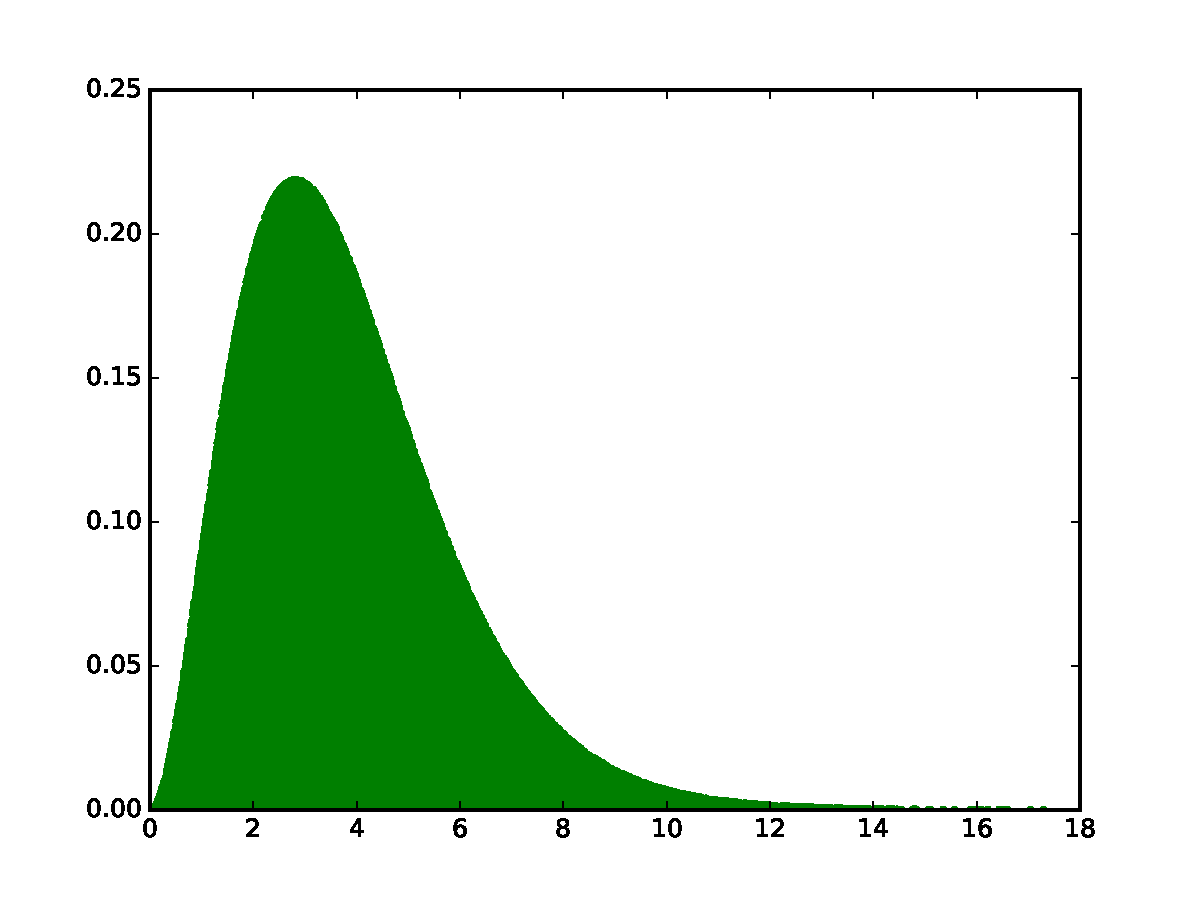
\includegraphics[height=7cm]{planck.pdf}
        \caption{Normale Rückweisungsmethode für die
        Planck-Funktion.}
        \label{fig:planck}
      \end{figure}

    \subsection{Aufgabe 1b}

      Hier soll ebenfalls das Rückweisungsverfahren angewendet werden.
      Allerdings wird nicht einfach ein Kasten um die Funktion gelegt wie in
      der Aufgabe 1a. Stattdessen wird nur um die Funktion
      im Intervall 0 bis $x_s$ ein Kasten mit oberer Grenze $y_{max}$ gelegt.
      Im zweiten Funktionsintervall von $x_s$ bis 20 wird die vorläufige
      $y-$Koordinate der Zufallszahlenpaare durch die obere Grenze
      \begin{align*}
        g(x) = 200Nx^{-0.1}\symup{exp}(-x^{0.9})
      \end{align*}
      beschränkt. \\
      Um den Schnittpunkt zwischen den beiden Majoranten zu berechnen, welcher
      gleichzeitig $x_s$ ist, setzt man die beiden Majorantenfunktionen gleich
      an der Stelle $x_s$ und berechnet somit (wieder mit scipy.optimize.brentq)
      die Nullstelle von
      \begin{align*}
        200Nx_s^{-0.1}\symup{exp}(-x_s^{0.9})-y_{max}\,\,\,.
      \end{align*}
      $N$ kann aus der Normierung von $g(x)$ gewonnen werden:
      \begin{align*}
        &\int_{x_s}^\infty g(x)dx = 1 = \left[-\frac{2000}9Ne^{-x^{9/10}}\right]_{x_s}^\infty\\
        \iff &N=\frac9{2000}e^{x_s^{9/10}}
      \end{align*}
      $x_s$ liegt ungefähr bei 5.68.\\

      Im Prinzip können mit der Kenntnis von $x_s$ beide Intervalle einzeln
      behandelt und im Anschluss zusammengefügt werden. \\
      Um eine einheitliche Dichte der Punkte zu gewährleisten,
      muss zunächst überprüft werden, auf welches Intervall wie viel Prozent
      der zur Verfügung stehenden Fläche entfallen. \\
      Gesamtfläche:
      \begin{align*}
        &\int_0^{x_s}y_{max}\,dx+\int_{x_s}^{20}g(x)\,dx\\
        =&x_sy_{max}+1
      \end{align*}
      Anteil von $N_1$: $\frac{x_sy_{max}}{1+x_sy_{max}} \implies 80\%$\\
      Anteil von $N_2$: $1-\frac{x_sy_{max}}{1+x_sy_{max}} \implies 20\%$\\
      Somit werden 80\% der $10⁵$ Punkte im linken Intervall verteilt und
      20\% im rechten.\\
      Nun ist es noch nötig, die Wahrscheinlichkeitsdichte von $g(x)$ zu bilden
      und diese zu invertieren, um eine gleichmäßige Verteilung unter dem
      Exponentialteil zu erhalten:
      \begin{align*}
        &\int_{x_s}^x g(x)dx=-e^{x_s^{9/10}}e^{-x^{9/10}}+1 = u\\
        \iff&x=\left(x_s^{9/10}-\symup{ln}(1-u)\right)^{10/9}
      \end{align*}

      Mithilfe dessen lassen sich die $10⁵$ Punkte nun plotten, was
      ein Bild ergibt wie in Abb. \ref{fig:majorante}.
      Der Plot unterscheidet sich optisch nicht vom Plot in Aufgabe 1a.



      \begin{figure}[H]
        \centering
        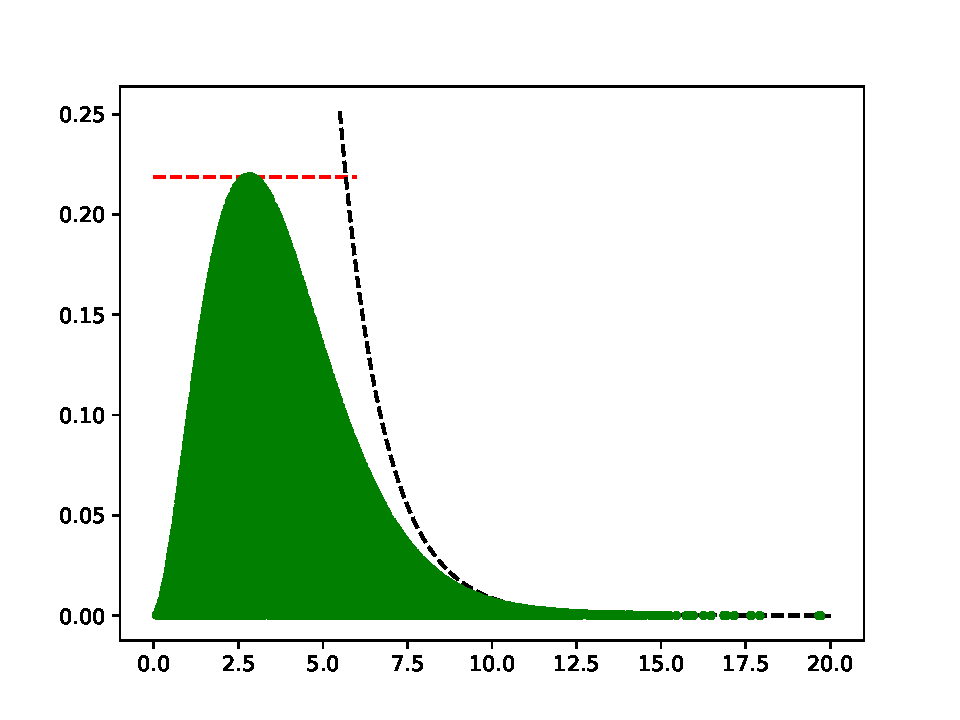
\includegraphics[height=7cm]{majorante.pdf}
        \caption{Rückweisungsmethode mit gestückelter Majorante.}
        \label{fig:majorante}
      \end{figure}




    \subsection{Aufgabe 1c}

      Die beiden Verfahren werden nun verglichen. \\
      Die erste Methode benötigt eine Rechenzeit von 0,071069\,s und
      muss während der Ausführung 337794 Werte zurückgeben, was ineffizient ist.\\
      Im Vergleich dazu benötigt die zweite Methode nur 0,027877\,s und
      muss nur 53390 Werte zurückgeben.\\
      Es ist natürlich logisch, dass die
      zweite Methode effizienter ist. Die Menge von Zufallszahlen, die
      zunächst erlaubt sind, aber nicht unter der Funktion liegen, ist beim
      ersten Verfahren wesentlich größer als beim zweiten.

\end{document}
